\documentclass[12pt,a4paper]{article}
\usepackage[MeX]{polski}
\usepackage[utf8]{inputenc}
\usepackage{hyperref}
\usepackage{amsmath}
\usepackage{pgfplots}
\usepackage{tikz}
\usepackage{braille}

\begin{document}
\title{Geometria punktu brajlowskiego w druku 3d w technologii FDM}
\author{Dawid Pieper \\ Fundacja Prowadnica}
\date{Maj 2023}
\maketitle

\begin{abstract}
Poniższy dokument przedstawia wyniki badań dotyczących możliwości wykonywania oznaczeń w alfabecie Brajla (zwanym inaczej pismem punktowym) z wykorzystaniem druku 3d w technologii FDM. Badanym zagadnieniem jest odpowiednie odwzorowanie geometrii punktu tak, by napis był w pełni czytelny dla osób niewidomych.
W pracy tej ujęte zostały modele matematyczne opisujące punkty Brajla oraz metodyka, która w trakcie testów mających miejsce od października 2021 roku została uznana za najbardziej obiecującą przez Zarząd Fundacji Prowadnica oraz niezależnych niewidomych testerów.

Celem niniejszego opracowania jest przedstawienie dokumentacji procesu i położenie fundamentów pod dalsze badania w tej dziedzinie.
Osoby pragnące wykonać tabliczki lub inne elementy z oznaczeniami w alfabecie Brajla z wykorzystaniem druku 3d mogą znaleźć skrócony wykaz zaleceń \hyperref[sec:recommendations]{na końcu niniejszej pracy}.
\end{abstract}

\newpage

\tableofcontents

\newpage

\section{Wstęp}
\emph{Fundacja Prowadnica} to organizacja, która za cel postawiła sobie, między innymi, badanie i promowanie wykorzystywania nowoczesnych technologii na rzecz osób niewidomych. Jednym z obszarów tych działań jest implementacja druku 3d w tworzeniu oznaczeń, makiet, materiałów edukacyjnych, gier planszowych i innych akcesoriów wykonywanych dla osób z dysfunkcją wzroku.
W ramach tych eksperymentów zbadana została także możliwość wykorzystania druku 3d do tworzenia oznaczeń w alfabecie Brajla.

Celem było sprawdzenie, czy możliwe jest tworzenie jakościowo akceptowalnych tabliczek z brajlowskimi podpisami z wykorzystaniem technologii FDM jako alternatywy do obecnie stosowanych, znacznie kosztowniejszych metod, a także samodzielne ich wykonywanie bezpośrednio przez instytucje, które zgłaszają zapotrzebowanie na tego typu oznaczenia.

W pracy tej zostały ujęte wyniki eksperymentów prowadzonych od października 2021 roku. Ponieważ stosowana w Fundacji technologia jest rozwijana w sposób ciągły, jeśli w badaniach wykazane zostaną dodatkowe czynniki lub zajdą istotne dla procesu zmiany, praca zostanie odpowiednio przeredagowana i wzbogacona o nowe treści.

\begin{figure}
\includegraphics[width=\linewidth]{sgn_pla.jpg}
\caption{Przykładowa tabliczka drukowana z PLA}
\end{figure}

\subsection{Przybliżenie terminologii i podstawowych zagadnień}
\subsubsection{Technologia FDM}
FDM (\emph{Fused Deposition Modelling}) to technologia druku 3D, w której model przestrzenny jest tworzony poprzez nakładanie kolejnych warstw topionego termoplastu. Proces drukowania odbywa się za pomocą dyszy, która przemieszcza się wzdłuż osi $x$ i $y$, tworząc ciąg linii w celu ukształtowania jednej warstwy modelu. Po ukształtowaniu każdej warstwy, dysza jest podnoszona i rozpoczyna się proces drukowania kolejnej. Technologia FDM cieszy się popularnością ze względu na swoją prostotę, szeroką gamę dostępnych materiałów oraz niskie wymagania. Jest też najpopularniejszą metodą druku 3d w zastosowaniach amatorskich.
Popularność technologii FDM stanowiła inspirację do przeprowadzenia badań nad możliwością jej wykorzystania do drukowania oznaczeń w alfabecie Brajla.

\subsubsection{Geometria FDM}
W związku z tematyką poruszaną w dalszej części niniejszego opracowania, warto rozważyć kwestię geometrii kształtów, które są wykonywane za pomocą technologii FDM.

Dysza drukarki 3d, uniesiona tuż nad powierzchnią stołu lub niższej warstwy, przepuszcza pewną ilość materiału, który formuje kształt zbliżony do walca o średnicy $d$ i wysokości $h$.
Średnica $d$ jest nazywana \emph{szerokością ścieżki ekstruzji}, zaś wysokość $h$ - \emph{wysokością warstwy}. Te parametry są kluczowe dla jakości druku, wraz z ich zmniejszaniem szczegółowość się poprawia.

Należy tu zauważyć, że w związku z geometrią druku 3d linia modelu nie jest prostopadłościanem, ale jego przybliżeniem złożonym z pewnej ilości walców. Efektem jest zaokrąglony kształt krawędzi tej linii. Zjawisko to jest tym wyraźniejsze, im większa jest szerokość ścieżki ekstruzji $d$, ta zaś jest zależna od średnicy stosowanej dyszy.
Pojedyncza warstwa powstaje z szeregu takich linii drukowanych w odległości $<d$ od siebie \cite{slicmath}.

Naturalnym następstwem podziału modelu na warstwy jest także zmniejszenie szczegółowości pionowej.
W rezultacie model zachowuje jedynie szczegółowość $h$ w osi $z$ oraz $\geq d$ w osiach $x$ i $y$.

\subsubsection{Alfabet Brajla}
Alfabet Brajla (Alfabet Braille'a) to wypukły zapis tekstu stosowany przez osoby niewidome. Pojedynczy znak tego alfabetu zawiera pewną kombinację punktów ułożonych w dwóch kolumnach i trzech rzędach, tak zwany sześciopunkt \cite{braille}. Punkty te w zapisie papierowym są wytłaczane dłutkiem lub na specjalnej maszynie brajlowskiej.
Sześciopunkty następnie organizuje się w wyrazy i wiersze analogicznie do pisma czarnodrukowego.
Należy tu podkreślić, że ze względu na ograniczoną liczbę kombinacji punktów $2^6=64$, istnieje kilka znaków specjalnych zmieniających znaczenie symbolów następujących po nich. Dodatkowo różne systemy zapisu Brajla zostały stworzone na potrzeby każdego języka. \cite{braillepolish} \cite{brailleenglish} .


\subsection{Metodyka badań}
W ramach badań wykonanych zostało ok. 1000 tabliczek, z których 585 zostało przekazanych do użytku w budynkach użyteczności publicznej.

Badane były tabliczki prostokątne o grubościach $1{,}0 \text{ mm}$, $2{,}0 \text{ mm}$, $3{,}0 \text{ mm}$, a także o nieregularnych kształtach (okręgi, elipsy, prostokąty o zaokrąglonych narożnikach).
Niektóre z tabliczek zawierały także kontrastową treść czarnodrukową, materiały graficzne lub kody QR.
Część z tabliczek była poddawana obróbce chemicznej.

Drukarki 3d wykorzystywane podczas badań:
\begin{itemize}
\item Original Prusa I3 MK3S+
\item Original Prusa I3 MK3S+ z MMU2S
\item Original Prusa Mini+
\end{itemize}

Wykorzystywane filamenty:
\begin{itemize}
\item Prusament PLA
\item Fiberlogy Easy PLA
\item Fiberlogy HD PLA
\item Rosa3D PLA Starter
\item Fiberlogy Easy ABS
\item Fiberlogy ABS Plus
\item Noctuo ABS
\item Noctuo ABS-MMA
\item Fiberlogy ASA
\item Devil Design PMMA
\item Fiberlogy FiberSilk
\item Rosa3D BioWOOD
\item Fiberlogy FiberFlex 40D
\item Fiberlogy Nylon PA12
\item Nebula Glass 807
\end{itemize}

Jeśli nie zaznaczono inaczej, stosowane były następujące ustawienia druku:
\begin{itemize}
\item Średnica dyszy; $0{,}4\text{ mm}$
\item Wysokość warstwy: $\in (0{,}07; 0{,}1) \text{ mm}$
\item Szerokość ścieżki: $0{,}45 mm$
\item Prędkość druku obrysów: $20 \text{mm/s}$
\end{itemize}

\section{Geometria punktu brajlowskiego}
W zagadnieniu druku 3d punktów Brajlowskich kluczowym problemem jest geometria pojedynczej kropki. Osoby niewidome odczytują tekst brajlowski poprzez dotykanie liter palcami. Oznacza to, że poprawne ukształtowanie i wykonanie punktów jest niezbędne dla uzyskania czytelności i użyteczności napisu.
Jak wspomniano powyżej, początkowo punkty brajlowskie były wykonywane z użyciem dłutka o zaostrzonej krawędzi, którym  naciskano na papier umieszczony na odpowiedniej tabliczce z niewielkimi, walcowymi otworami. Tabliczkę profilowano w taki sposób, by punkt stał się wyraźny w dotyku na powierzchni kartki, ale by sama kartka nie została przebita.
Taki punkt ma zaokrąglony kształt, nie jest walcem, stożkiem czy kulą.
Punkt brajlowski definiowany jest przez średnicę podstawy $d$ oraz wysokość $h$. Dla specyfikacji Marburg Medium \cite{brailleiso} są to odpowiednio:

$d \in (1{,}3; 1{,}6) \text{ mm}$,

$h = (0{,}5 \pm 0{,}1) \text{ mm}$.

Można przyjąć, że punkt brajlowski jest figurą powstałą poprzez obrót półelipsy o półosiach $d/2$ i $h$ wokół półosi $h$.

\begin{figure}
\centering
\begin{tikzpicture}
\def\a{0.65}
\def\b{0.5}
\draw[dashed] (0,0) arc (180:360:{\a} and {\b});
\draw[dotted] (-\a,0) -- (\a,0) node[right]{$d$};
\draw[dotted] (0,0) -- (0,\b) node[above]{$h$};
\end{tikzpicture}
\caption{Przekrój prostopadły punktu brajlowskiego}
\end{figure}

Równanie tej elipsoidy przyjmuje następującą postać:
\begin{figure}
Dla każdego $z \geq 0$

$4\frac{x^2+y^2}{d^2} + \frac{z^2}{h^2} \leq 1$,

gdzie $x$, $y$ i $z$ są współrzędnymi punktu.
\caption{Równanie elipsoidy punktu brajlowskiego}
\end{figure}

Komputerowe uzyskanie punktu możliwe jest na dwa podstawowe sposoby.

\subsection{Punkt brajlowski jako skalowana półkula}
Dana jest półkula o środku w punkcie $(0;0;0)$ i promieniu $d.2$, czyli wyrażona równaniem

Dla każdego $z \geq 0$

$4\frac{x^2+y^2+z^2}{d^2} \leq 1$,

gdzie $x$, $y$ i $z'$ są współrzędnymi punktu.

Poprzez wykorzystanie skalowania można w łatwy sposób uzyskać pożądaną geometrię punktu brajlowskiego. Wystarczy przyjąć współczynniki skalowania
$$
\begin{bmatrix}
1 & 0 & 0 \\
0 & 1 & 0 \\
0 & 0 & \frac{h}{d}
\end{bmatrix}
$$

Ponieważ dla $x,y \in (-d/2; d/2)$

$z = \sqrt{\frac{d^2}{4} - x^2 - y^2}$,

Uzyskujemy wzór skalowania


\begin{figure}
$z' = \frac{h*2}{d} \sqrt{\frac{d^2}{4} - x^2 - y^2}$,

gdzie $z'$ jest współrzędną osi $z$.
\caption{Skalowanie półkuli do półelipsoidy punktu Brajlowskiego}
\end{figure}

\subsubsection{Przykład implementacji}
Poniżej znajduje się przykładowa implementacja w języku OpenSCAD.

\begin{figure}
\begin{verbatim}
module brailleDot(d, h) {
  scale([1, 1, h/d])
    difference() {
      sphere(d=d);
      translate([0, 0, -d/2])
        cylinder(d=d, h=d/2);
    }
}
\end{verbatim}
\caption{OpenSCAD: reprezentacja punktu brajlowskiego poprzez skalowanie kuli}
\end{figure}

\subsection{Punkt Brajlowski jako wycinek kuli}
Ponieważ jakość powyższego przekształcenia jest silnie związana z przyjętą rozdzielczością skalowania i mało zoptymalizowana, można również ująć punkt brajlowski jako zbiór punktów kuli o środku w punkcie $z<0$ takich, że $z \geq 0$.

Dana jest kula o promieniu $R>d/2$ o środku w punkcie $z<0$.
Kula ta posiada punkt o współrzędnych $(0;0;h)$, a jej płaszczyzną w wysokości $z=0$ jest okrąg o promieniu $d/2$.
Promień tej kuli będzie także promieniem koła stanowiącego przekrój tej kuli.

Dane jest koło o promieniu $R$ ze środkiem w punkcie $y<0$.
W kole wyznaczone zostały punkty:
\begin{itemize}
\item $P$: $(0; 0)$,
\item $A$: $(-d/2; 0)$,
\item $B$: $(d/2; 0)$,
\item $C$: $(0; h)$,
\item $D$: $(0; h-2R)$.
\end{itemize}

Wytyczone zostały cięciwa $\overline{AB}$ oraz średnica $\overline{CD}$ przecinające punkt $P$.

\begin{figure}
\centering
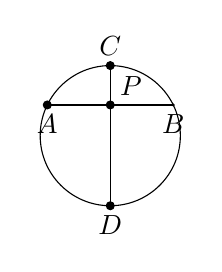
\begin{tikzpicture}
\draw (0,-0.39) circle [radius=0.89];
\filldraw (0,0) circle [radius=0.05] node [above right] {$P$};
\filldraw (-0.8,0) circle [radius=0.05] node [below] {$A$};
\filldraw (0.8,0) circle [radius=0.01] node [below] {$B$};
\filldraw (0,0.5) circle [radius=0.05] node [above] {$C$};
\filldraw (0,-1.28) circle [radius=0.05] node [below] {$D$};
\draw (-0.8,0) -- (0.8,0);
\draw (0,-1.28) -- (0,0.5);
\end{tikzpicture}
\caption{Koło rozważane przy analizie elipsy prostopadłego przekroju punktu brajlowskiego}
\end{figure}

$ \left| PA \right| = \left| PB \right| = \frac{d}{2}$, ponieważ punkt $P$ leży na średnicy koła.

\emph{Twierdzenie o Cięciwach} \cite{chords} mówi, że

\begin{figure}
Jeśli w okręgu 2 cięciwy $\overline{AB}$ i $\overline{CD}$ przecinają się w punkcie $P$,
$ \left|PA\right| \times \left| PB \right| = \left| PC \right| \times \left| PD \right| $.
\caption{Twierdzenie o cięciwach}
\end{figure}

Możemy stąd wyznaczyć długość odcinka
$\overline{PD} = \frac{\frac{d}{2} * \frac{d}{2}}{h}$.

$$
R = \frac{\overline{PC} + \overline{PD}}{2} =
\frac{h + \frac{\frac{d}{2} * \frac{d}{2}}{h}}{2} = \\
\frac{h + \frac{d^2}{4h}}{2} = \\
\frac{h + \frac{d^2}{4h}}{2} = \\
\frac{h + \frac{d^2}{4h}}{2}
$$

Zatem punkt Brajlowski może być stworzony jako fragment kuli $z \geq 0$ o promieniu $R$ i środku w punkcie $P$.

Równanie tego punktu przyjmuje postać:

\begin{figure}
Dla każdego $z>0$

$x^2 + y^2 + (z - z_P)^2 = R^2$,

gdzie:

$R = \frac{h + \frac{d^2}{4h}}{2}$,

$z_P = h-R$.
\caption{Równanie półelipsoidy punktu brajlowskiego wyznaczonej z kuli}
\end{figure}

Powyższa formuła będzie stosowana celem uproszczenia obliczeń w dalszej części niniejszego opracowania, ale należy pamiętać, że obydwie zaprezentowane strategie są tożsame.

\subsubsection{Przykład implementacji}
Poniżej znajduje się przykładowa implementacja w języku OpenSCAD.

\begin{figure}
\begin{verbatim}
function calculateDotSphereRadius(d,h) = 
  (d^2 / (4*h) + h) / 2;

module brailleDot(d, h) {
  rk = calculateDotSphereRadius(d, h);
  difference() {
    translate([0, 0, h-rk])
      sphere(r=rk);
    translate([0, 0, h-rk*2])
      cylinder(r=rk, h=rk*2-h);
    }
}
\end{verbatim}
\caption{OpenSCAD: reprezentacja punktu brajlowskiego jako półelipsoidę będącą wycinkiem kuli}
\end{figure}

\subsection{Układ punktów}
Prócz wymiarów odnoszących się do samego punktu, czcionka Brajlowska definiuje także odległość między punktami w jednym znaku ($o$), odległość między sąsiednimi znakami ($w$) oraz wysokość linii tekstu ($l$).
Dla czcionki Marburg Medium są to:
\begin{itemize}
\item $o = 2{,}5 \text{ mm}$
\item $w = 6{,}0 \text{ mm}$
\item $l = 10{,}0 \text{ mm}$
\end{itemize}

Przykładowo w Brajlu słowo "test" ma postać: \braille{test}.

Poniższy kod w języku OpenSCAD pozwoli na stworzenie tego napisu.

\begin{figure}
\begin{verbatim}
module writeBraille(letters, o=2.5, w=6.0, l=10.0, d=1.3, h=0.5) {
  for(line = [0: len(letters)-1]) {
    translate([0, -l*line-l/2, 0]) {
      for(char = [0: len(letters[line])-1]) {
        translate([char*w+w/2, 0, 0])
          letter = letters[line][char];
          for(point = [0: len(letters[line][char])-1]) {
          x = floor(point/3)*o - o/2;
          y = floor((point-1)%3)*o - o;
          translate([x, y, 0])
            brailleDot(d, h)
          }
      }
    }
  }
}

// Przyjmuje się, że w Brajlu punkty numerowane są od góry: (1, 2, 3 - pierwsza kolumna; 4, 5, 6 - druga)
letters = [[[2,3,4,5], [1,5], [2,3,4], [2,3,4,5]]];
writeBraille(letters);
\end{verbatim}
\caption{OpenSCAD: przykładowy napis w Brajlu}
\end{figure}

\section{Reprezentacja geometrii druku FDM punktu ułożonego równolegle do powierzchni stołu}

Przez $H$ oznaczmy wysokość warstwy druku FDM, $D$ szerokość ścieżki ekstruzji, $h_p$ wysokość punktu Brajlowskiego, a $d_p$ średnicę podstawy.
$D$ oznacza minimalną średnicę walca umieszczanego na warstwie druku. Należy zauważyć, że rzeczywista wytłaczana średnica jest skwantowana do wielokrotności $D$ w przedziale $(0, D \cdot 2)$, ponieważ nie jest możliwe umieszczenie linii składającej się z niepełnej szerokości ścieżki.
Warto nadmienić, że w rzeczywistości współczesne oprogramowanie stara się dynamicznie dostosować szerokość ścieżki do potrzeb, będąc w stanie lekko ją zwężać lub rozszerzać \cite{arachne}. Jest to stosunkowo nowe podejście, jednak dla uproszczenia obliczeń w niniejszej pracy założona zostanie stała wartość $D$, nowość ta nie ma większego wpływu na poprawne drukowanie Brajla, gdyż rzeczywiste różnice w szerokości ścieżki są zbyt niewielkie.

Zależność średnicy walca składającego się na punkt $d_z$ od wysokości $z$ przedstawia wzór

\begin{figure}
$d_z = 2 * \sqrt{(R_k)^2 - (R_k - h_p + z)^2}$,

gdzie $R_k = \frac{h_p + \frac{d_p^2}{4h_p}}{2}$
\caption{Średnica równoległego przekroju punktu Brajlowskiego na wysokości $z$}
\end{figure}

Na poniższym wykresie zaznaczone są poprawne średnice walców czerwona linia) i rzeczywiste średnice niebieska linia) na kolejnych warstwach dla $d_p = 1{,}3 \text{ mm}$ i $h_p = 0{,}5 \text{ mm}$.

\begin{figure}
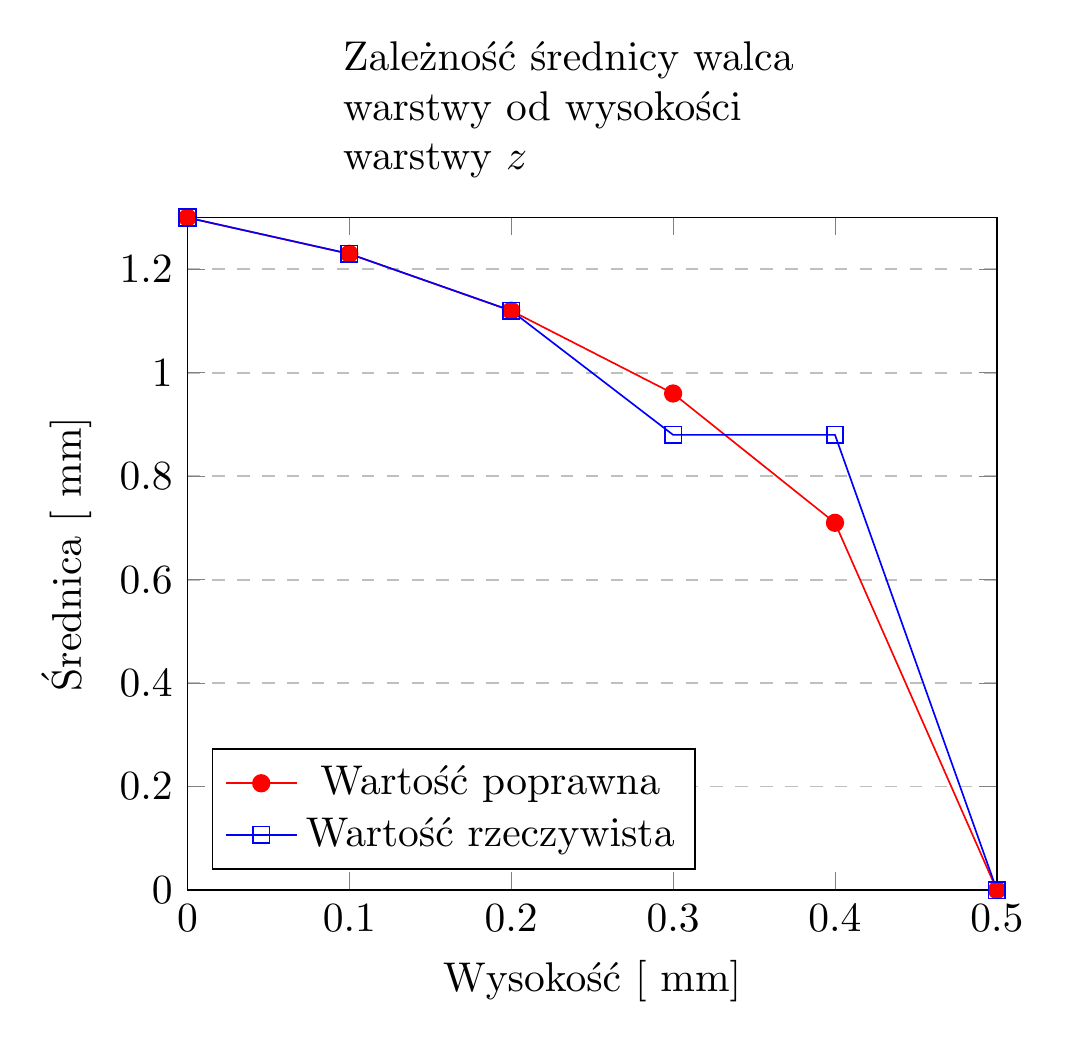
\begin{tikzpicture}[scale=1.5]
\begin{axis}[
title={Zależność średnicy walca warstwy od wysokości warstwy $z$},
title style={text width=12em},
xlabel={Wysokość [\text{ mm}]},
ylabel={Średnica [\text{ mm}]},
xmin=0.0,xmax=0.5,
ymin=0.0,ymax=1.3,
legend pos=south west,
ymajorgrids=true,grid style=dashed
]
\addplot[color=red,mark=*]
coordinates {
(0,1.3)
(0.1,1.23)
(0.2,1.12)
(0.3,0.96)
(0.4,0.71)
(0.5,0.0)
};
\addplot[color=blue,mark=square]
coordinates {
(0,1.3)
(0.1,1.23)
(0.2,1.12)
(0.3,0.88)
(0.4,0.88)
(0.5,0)
};
\legend{Wartość poprawna,Wartość rzeczywista}
\end{axis}
\end{tikzpicture}
\caption{Wykres porównujący rzeczywistą i drukowaną średnicę punktu Brajlowskiego ustawionego równolegle do powierzchni druku}
\end{figure}

Powstały kształt nie jest sferyczny. W skutek niskiej rozdzielczości przy tak małej skali w wyniku otrzymuje się nieregularny, szpiczasty stożek. Efekt ten jest jeszcze potęgowany przez wyciekanie nadmiarowego filamentu z dyszy.
Uzyskiwany tym sposobem Brajl jest kłujący, nieprzyjemny w dotyku i trudny do odczytywania.
Z powodu szerokiej ścieżki ekstruzji, zmniejszanie wysokości warstwy nie ma wpływu na zaistniałą sytuację, od punktu $z \approx 0,34$ średnica wytłaczanego walca na warstwie będzie kwantowana.

\begin{figure}
\centering
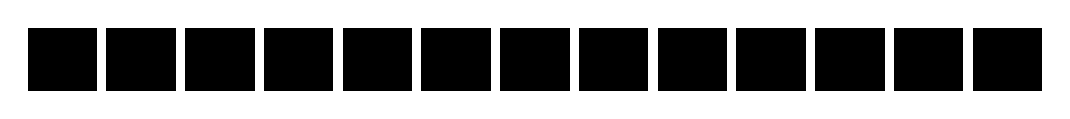
\begin{tikzpicture}
\def\h{0.1}
\def\w{1.3, 1.22, 1.12, 0.95, 0.88}
\foreach \i in {0,1,...,12} {
\filldraw[black] (\i-\w[\i]/2, \i*\h) rectangle ++(\w[\i], \h);
}
\end{tikzpicture}
\caption{Przekrój poziomy punktu o wymiarach $h_p = 0{,}5 \text{ mm}$ i średnicy podstawy $d_p=1{,}3 \text{ mm}$ drukowanego równolegle przy wysokości warstwy $H = 0{,}1 \text{ mm}$ i szerokości ścieżki $D = 0{,}45 \text{ mm}$}
\end{figure}

Sytuacje może poprawić stosowanie dysz o niższej średnicy, co spowoduje mniejszą szerokość ścieżki ekstruzji, ale dopiero wartości $D \leq 0{,}2 \text{ mm}$ pozwolą na odwzorowanie kształtu kropki z dokładnością do $0{,}05 \text{ mm}$, odpowiada to dyszomo średnicy $0{,}15 \text{ mm}$, których stosowanie jest znacznie trudniejsze od standardowych i wiąże się ze znacznym wydłużeniem czasu druku i ograniczeniem puli dostępnych materiałów \cite{e3d15}.

\section{Reprezentacja geometrii druku FDM punktu prostopadłego do powierzchni stołu}
Sytuacja przedstawia się zupełnie inaczej, gdy punkty drukowane są prostopadle do powierzchni stołu. W tym przypadku kolejne warstwy stają się półelipsami.

Dla uproszczenia rozważmy geometrię punktów w takim samym układzie współrzędnych jak poprzednio, czyli niech wysokość punktu odpowiada osi $z$. W tej sytuacji punkt będzie dzielony w osi $y$, a kolejne warstwy będą zawierać połowę walca eliptycznego.

Należy wyznaczyć półosie tej elipsy.
Elipsoida punktu dana jest wzorem
$(x^2 / \frac{d_p}{2}^2) + (y^2 / \frac{d_p}{2}^2) + (z^2 / h_p^2) = 1$.

Równanie opisujące elipsę stanowiącą przekrój w osi $y$ w odległości $l$ od środka przyjmuje postać
$(x^2 / \frac{d_p}{2}^2) + (z^2 / h^2) = (1 - l^2 / \frac{d_p}{2}^2),$
z czego można wyprowadzić wartość z

$$
z^2 = h_p^2 * (1 - (x^2 / \frac{d_p}{2}^2)) = \\
h_p^2 * (1 - ((\frac{d_p}{2}^2 - l^2) / \frac{d_p}{2}^2)) = \\
h_p^2 * (l^2 / \frac{d_p}{2}^2)
$$

Zatem, półosi elipsy w odległości $l$ od środka to:

\begin{figure}
$$
d_l = 2 * \sqrt(\frac{d_p}{2}^2 - l^2) \\
h_l = h_p * \sqrt(l^2 / \frac{d_p}{2}^2)
$$,

gdzie $d_l$ to oś elipsy w osi $x$, a $h_p$ półoś elipsy w osi $z$.
\caption{Wielkość półosi elipsy przekroju prostopadłego punktu brajlowskiego w odległości $l$ od środka}
\end{figure}

Przenosząc powyższe w geometrię druku, należy zauważyć, że wartość $h_p$ nie ma znaczenia podczas druku, o ile tylko szerokość obiektu, na którym nanoszony jest napis, wynosi $\geq D*2$. Pozwala to wykonać punkt z wykorzystaniem przestrzeni wewnątrz modelu.
Zatem na rozdzielczość punktu wpływ ma jedynie wartość $d_l$ (szerokość ścieżki) oraz wysokość warstwy$H$.

Na poniższym wykresie zaznaczone są poprawne osie elips czerwona linia) i rzeczywiste osie niebieska linia) na kolejnych warstwach dla $d_p = 1{,}3 \text{ mm}$ i $h_p = 0{,}5 \text{ mm}$ dla odległości $l$ względem środka elipsy.

\begin{figure}
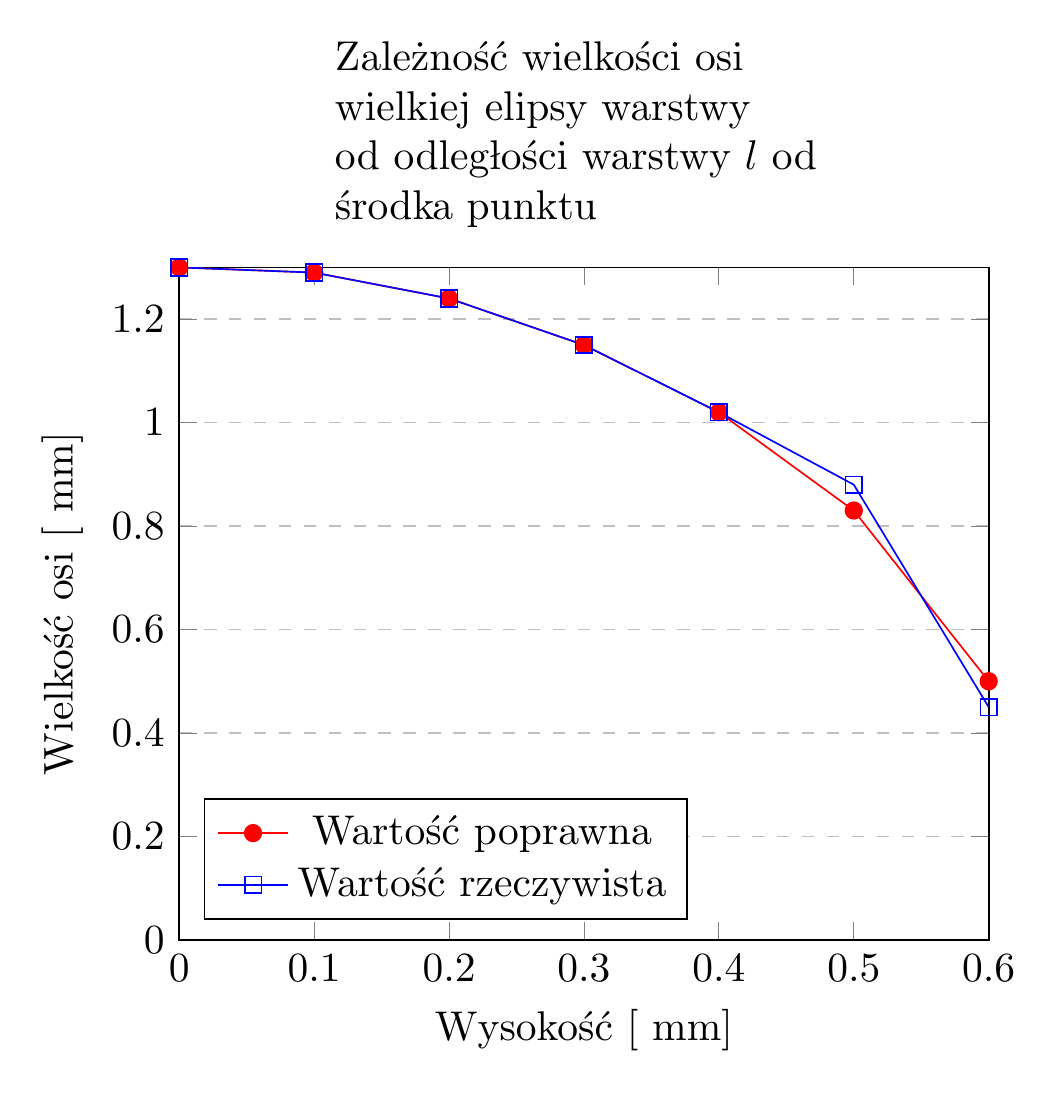
\begin{tikzpicture}[scale=1.5]
\begin{axis}[
title={Zależność wielkości osi wielkiej elipsy warstwy od odległości warstwy $l$ od środka punktu},
title style={text width=12em},
xlabel={Wysokość [\text{ mm}]},
ylabel={Wielkość osi [\text{ mm}]},
xmin=0.0,xmax=0.6,
ymin=0.0,ymax=1.3,
legend pos=south west,
ymajorgrids=true,grid style=dashed
]
\addplot[color=red,mark=*]
coordinates {
(0,1.3)
(0.1,1.29)
(0.2,1.24)
(0.3,1.15)
(0.4,1.02)
(0.5,0.83)
(0.6,0.5)
};
\addplot[color=blue,mark=square]
coordinates {
(0,1.3)
(0.1,1.29)
(0.2,1.24)
(0.3,1.15)
(0.4,1.02)
(0.5,0.88)
(0.6,0.45)
};
\legend{Wartość poprawna,Wartość rzeczywista}
\end{axis}
\end{tikzpicture}
\caption{Wykres porównujący zależność wielkości osi wielkiej elipsy warstwy od odległości warstwy $l$ od środka punktu w druku prostopadle do powierzchni}
\end{figure}

Odwzorowanie geometrii punktu Brajlowskiego nawet dla standardowej szerokości ścieżki jest o wiele wierniejsze, niż w poprzednim przykładzie. Można je jeszcze bardziej zwiększać, poprzez zmniejszanie wysokości warstw.

\begin{figure}
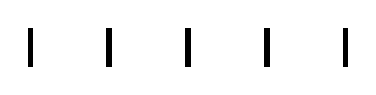
\begin{tikzpicture}
\def\h{0.1}
\def\w{0.45, 0.88, 1.02, 1.15, 1.24, 1.29, 1.3, 1.29, 1.24, 1.15, 1.02, 0.88, 0.45}
\foreach \i in {0,1,...,4} {
\filldraw (\i-\w[\i]/2, \i*\h) rectangle ++(\w[\i], \h);
}
\end{tikzpicture}
\caption{Przekrój pionowy punktu o wymiarach $h_p = 0{,}5 \text{ mm}$ i średnicy podstawy $d_p=1{,}3 \text{ mm}$ drukowanego prostopadle przy wysokości warstwy $H = 0{,}1 \text{ mm}$ i szerokości ścieżki $D = 0{,}45 \text{ mm}$}
\end{figure}

Zgodnie z eksperymentami wykonywanymi przez Fundację Prowadnica od października 2021 roku, Brajl staje się czytelny już przy wysokości warstwy $H \leq 0{,}2 \text{ mm}$. Uznany przez Fundację Prowadnica najlepszy stosunek wysokości warstwy do jakości to $H \in (0{,}07; 0{,}1) \text{ mm}$.

Dodatkowym atutem tej geometrii jest zwiększona odporność punktów na ścieranie - nie stanowią one osobnej warstwy, ale są częścią warstw modelu, na którym są umieszczone.

\begin{figure}
\includegraphics[width=\linewidth]{sgn_printed.jpg}
\caption{Tabliczka z PLA drukowana prostopadle, wysokość warstwy $0{,}07 \text{ mm}$}
\end{figure}

\section{Pozostałe czynniki mające wpływ na geometrię punktów}
\subsection{Struktura materiału}
Warto zauważyć, że choć na czytelność Brajla największy wpływ ma jego orientacja względem płaszczyzny druku, rozważany model elipsoidy nie w pełni oddaje wygląd prawdziwego, tłoczonego Brajla. W rzeczywistości kształt punktów jest nieregularny.
Zaprezentowany model matematyczny Brajla doskonale nadaje się do oznaczeń i tyflografik. W trakcie prowadzonych eksperymentów udało się jednak uzyskać nawet wierniejszą geometrię.
Wpływ na to ma dobór odpowiedniego materiału. Testowane były między innymi filamenty składające się z włókien drewnianych. Charakterystyką tych materiałów jest niejednorodna struktura, która sprawia, że grubość ścieżek jest nieregularna. Wytwarzany w ten sposób Brajl okazywał się o wiele bardziej zbliżony do punktów umieszczanych na kartce metodami tradycyjnymi.

\begin{figure}
\includegraphics[width=\linewidth]{sgn_wood.jpg}
\caption{Tabliczka z włóknami drewnianymi drukowana prostopadle, wysokość warstwy $0{,}07 \text{ mm}$}
\end{figure}

\subsection{Temperatura dyszy}
Wraz z temperaturą dyszy zwiększa się nadmiarowe wyciekanie materiału \cite{3dparameters}. Gromadzący się w ten sposób materiał na punktach Brajlowskich, niezależnie od przyjętej geometrii, powoduje pogorszenie ich właściwości geometrycznych.
W trakcie testów wykorzystany został polilaktyd produkcji firmy "Prusa Research" ("Prusament PLA") oraz "Fiberlab S.A." ("Fiberlogy FiberSilk"). Wykonanych zostało po 10 tabliczek z każdego z tych materiałów w temperaturach: $200^{\circ} C$, $215^{\circ} C$ oraz $230^{\circ} C$. Badanie zostało przeprowadzone na drukarce 3d "Original Prusa I3 MK3S+" z wykorzystaniem oryginalnego hotendu "E3D Hotend V6".
Podczas gdy tabliczki w temperaturze $200^{\circ} C$ były niemal bezbłędne, ich łączenie warstw było najsłabsze i z łatwością dało się je połamać w osi $z$. Analogicznie tabliczki wykonane w temperaturze $230^{\circ} C$ były najtrwalsze, ale punkty Brajla charakteryzowały się ostrością spowodowaną nadmiernym wypływaniem filamentu, ich czytanie uznane zostało za mniej przyjemne w stosunku do pozostałych. Dlatego przyjęto, że temperatura $215^{\circ} C$ stanowi dobry kompromis jakości i wytrzymałości elementów, choć należy podkreślić, że czasem na tabliczkach tych pojawiają się różnego rodzaju artefakty.

\subsection{Wpływ warunków zewnętrznych na jakość i geometrię punktu}
Ocena wpływu warunków zewnętrznych na jakość samego punktu jest trudna, ale najprawdopodobniej wpływ ten pozostaje pomijalny z powodu bardzo niewielkich rozmiarów pojedynczej kropki. W rzeczywistości jednak wpływ na sam punkt, szczególnie podczas druku prostopadłego, mają nieprawidłowości powstałe w modelu, na którym jest on umieszczany - wypaczenia, problemy z adhezją, niedostateczna lub nadmierna ekstruzja powodują deformację, przesunięcia lub nieczytelność Brajla.
Materiały podatne na wypaczenie, takie jak terpolimer akrylonitrylo-butadieno-styrenowy (ABS), poliamidy lub poliwęglany powinny być drukowane w odpowiednich dla nich warunkach. Brajl pozostaje też podatny na niedostateczne chłodzenie modelu, w przypadku druku cienkich tabliczek z polimerów topionych w wysokich temperaturach przy nadmiernej prędkości druku zaobserwować można rozlanie kropki Brajla na zbyt dużym obszarze.

\subsection{Prędkość druku}
Prędkość druku zazwyczaj ma ogromny wpływ na jakość. W przypadku Brajla jest podobnie.
Zazwyczaj jednak w druku FDM stosuje się bardzo zaniżoną prędkość obrysów w stosunku do reszty modelu. Ponieważ w druku Brajla prostopadle do powierzchni stołu cała wypukła część kropki jest obrysem, możliwe jest poprawne drukowanie modeli z nawet bardzo dużą prędkością wypełnienia. Należy mieć jednak na względzie, że błędy w samym modelu mają wpływ także na Brajla, szczególnie w przypadku deformacji części. Dodatkowo tabliczki o niskiej grubości zazwyczaj są zbyt małe, by posiadać rzeczywiste wypełnienie, tabliczka o grubości $2 \text{ mm}$ dla szerokości ścieżki $d=0{,}45 \text{ mm}$ będzie się składać jedynie z dwóch obrysów i jednej linii wewnątrz modelu.
Testowane były także różne możliwości zmniejszania czasu druku:
\begin{itemize}
\item Tworzenie wypełnienia o większej wysokości warstwy w stosunku do obrysu praktycznie nie ma wpływu na jakość Brajla, nie udało się zaobserwować znaczących różnic,
\item Drukowanie tabliczek posiadających tylko jeden obrys nawet dla standardowej dyszy $0{,}4 \text{ mm}$ powodowało przezieranie wypełnienia na obrysie i deformację Brajla podczas użytkowania zarówno w przypadku polilaktydu (PLA), jak poliamidu,
\item Drukowanie tabliczek w trybie wazy daje zaskakująco dobre efekty, choć powstające w ten sposób modele charakteryzują się bardzo niską wytrzymałością,
\item Drukowanie kilku tabliczek jednocześnie jest możliwe, ale należy dostosować ustawienia retrakcji, gdyż typowym zjawiskiem są nitki materiału powstające między kilkoma modelami na stole.
\end{itemize}

\subsection{Wygładzanie chemiczne}
Jakość modeli wytwarzanych metodą FDM można znacznie poprawić przez różnego rodzaju obróbkę, jednym z przykładów jest wygładzanie chemiczne.
Proces ten polega na umieszczeniu wykonanego modelu w oparach rozpuszczalnika (czasem wręcz zanurzeniu lub pokryciu go nim). W rezultacie poprzez częściowe rozpuszczenie materiału można zniwelować widoczność i rozgraniczenie pojedynczych warstw \cite{postprocessing}.

Doświadczenie polegało na umieszczaniu tabliczek (Brajlem do dołu) na pewnej wysokości szklanego naczynia w kształcie stożka. Na dole naczynia znajdowało się $50 \text{ ml}$ odpowiedniej substancji.  W trakcie badań tabliczki wykonywane z terpolimeru akrylonitrylo-butadieno-styrenowego (ABS) były umieszczane w oparach acetonu, a te wykonane z polilaktydu (PLA) w oparach dichlorometanu i metyloetyloketonu (MEK).
Substancje te były następnie podgrzewane do temperatury zbliżonej do temperatury wrzenia: odpowiednio:
\begin{itemize}
\item Aceton: $85^{\circ} C$
\item Dichlorometan: $35^{\circ} C$
\item MEK: $75^{\circ} C$
\end{itemize} 

Okazało się, że wygładzanie chemiczne nadaje równy, sferyczny kształt punktom brajlowskim, nawet tym wykonanym równolegle do powierzchni stołu. Kluczowe jest jednak odpowiednie dobranie czasu - zbyt krótkie wygładzanie nie daje zadowalających efektów, a zbyt długie powoduje całkowitą utratę punktów i tabliczki.
Wyniki doświadczeń prezentowały się następująco, dla tabliczek o grubości $2 \text{ mm}$:
\begin{table}[t]
\caption{Wyniki doświadczeń polegających na wygładzaniu chemicznym tabliczek}
\begin{tabular}{|l|l|l|l|l|l|l|}
\hline
Substancja & Efekt po 5 minutach & Efekt po 8 minutach & Efekt po 12 minutach & Efekt po 15 minutach & Efekt po 20 minutach & Efekt po 25 minutach \\
\hline
ABS, aceton & Nadanie lekkiego połysku, brak wyraźnych zmian & Nadanie wyraźnego połysku, brak zmian geometrii Brajla & Kropki Brajla lekko wygładzone & Kropki Brajla w kształcie sferycznym & Kropki Brajla zbyt wygładzone, trudne do odczytania & Kropki Brajla niemożliwe do odczytania \\
\hline
PLA, MEK & Brak obserwowalnych zmian & Lekkie wygładzenie linii, brak zmian geometrii punktów & Kropki Brajla lekko wygładzone, obserwowane deformacje tabliczki & Kropki Brajla w kształcie sferycznym, tabliczka wyraźnie zdeformowana & Tabliczka wyraźnie zdeformowana, utrata kropek & Tabliczka wyraźnie zdeformowana, utrata kropek \\
\hline
PLA, dichlorometan & Kropki Brajla lekko wygładzone & Kropki Brajla w kształcie sferycznym, linie wyrównane & Kropki Brajla trudne do wyczucia, tabliczka bardzo wygładzona & Tabliczka ulega deformacji & Tabliczka uszkodzona & Tabliczka uszkodzona \\
\hline
\end{tabular} 
\end{table}

W testowanej konfiguracji idealne czasy wynosiły 15 minut dla acetonu oraz 8 minut dla dichlorometanu.
Wadą procesu jest jednak nadmierne wygładzenie wykończenia punktów, co utrudnia ich odczytanie na przykład na zewnątrz w zimniejsze dni. Dlatego decyzja o wykorzystaniu tej metody powinna być uzależniona od przeznaczenia oznaczeń.

Warto też wspomnieć, że wygładzanie chemiczne pozwala na uzyskiwanie przezroczystych wydruków z materiałów takich jak polimetakrylan metylu (PMMA), dzięki czemu możliwe jest stosowanie poddruku poniżej warstw przezroczystego Brajla.

\begin{figure}
\includegraphics[width=\linewidth]{sgn_underprint.jpg}
\caption{Tabliczka drukowana równolegle, z poddrukiem i wygładzona chemicznie}
\end{figure}

\section{Trwałość oznaczeń wykonywanych w technologii FDM}
Wytrzymałość oznaczeń wykonywanych w technologii FDM jest uzależniona od wielu czynników, ale najważniejszym z nich jest dobór odpowiedniego materiału.
Przykładowo polilaktyd (PLA) charakteryzuje się temperaturą zeszklenia już w granicy $\in (40; 60)^{\circ} C$, a także niską odpornością na promieniowanie UV, co wyklucza go ze stosowania w oznaczeniach na zewnątrz budynków, w szczególności w silnie nasłonecznionych miejscach. Z drugiej strony terpolimer akrylonitryl-styren-akryl (ASA) charakteryzuje się temperaturą zeszklenia $\in (80; 105)^{\circ} C$ i niemal całkowitą odpornością na promieniowanie ultrafioletowe \cite{plaabsasa}.

W przypadku geometrii punktu drukowanego prostopadle do powierzchni stołu, kropki stają się elementem obrysu, którego przedłużeniem jest element, na którym nanoszone są oznaczenia. W rezultacie nie występuje efekt osłabienia materiału na łączeniu warstw.

W 2021 roku Fundacja Prowadnica zorganizowała konkurs \emph{Właściwe Drzwi}, w ramach którego darmowo wykonanych zostało 585 tabliczek z materiału "Prusament PLA" firmy "Prusa Research", przekazanych nieodpłatnie do 10 budynków użyteczności publicznej, w tym dla szpitala, muzeum, urzędów czy placówek edukacyjnych. Tabliczki te były instalowane w okresie od grudnia 2021 roku do sierpnia 2022 roku. Na kwiecień 2023 roku nie stwierdzono wypaczenia lub uszkodzenia żadnej z nich. Stan tych oznaczeń będzie dalej monitorowany.

\section{Obszary dalszych badań}
\subsection{Druk nieplanarny}
W 2019 roku naukowcy z Uniwersytetu w Hamburgu w Niemczech zaproponowali zmianę podejścia do druku FDM \cite{nonplanar}. Jak wyjaśniono na początku opracowania, druk FDM polega na umieszczaniu kolejnych warstw topionego termoplastu. Zaproponowane nowe podejście, nazwane \emph{drukiem nieplanarnym} polega na wykorzystaniu rzeczywistych, trójwymiarowych ruchów dyszy drukarki 3d do uzyskania gładkich, okrągłych powierzchni. Jest to osiągane poprzez wykonywanie jednoczesnych ruchów dyszy we wszystkich trzech osiach.
Ta koncepcja może potencjalnie pozwolić na znaczną poprawę jakości drukowanego Brajla, w a/szczególności w układzie równoległym do powierzchni stołu. Znacznie ułatwiłoby to wykorzystanie druku FDM do tworzenia dużych makiet tyflograficznych.
W takiej sytuacji punkt Brajlowski mógłby być tworzony z perspektywy dwuwymiarowej jako koło o średnicy $d_p$, odpowiedni kształt punktu byłby zaś nadawany jedynie poprzez ciągłą zmianę wysokości osi $z$.

Wysokość $z$ danego obszaru względem środka punktu dana jest wzorem:

\begin{figure}
$z(x,y) = h_p * \sqrt{1 - \frac{x^2+y^2}{\frac{d_p}{2}^2}}$.
\caption{Wysokość punktu w punkcie $x$, $y$ względem środka elipsoidy}
\end{figure}

Kwestią dalszych badań pozostaje zagadnienie rozdzielczości. W szczególności elipsoida punktu podzielona zostanie na $\approx d_p/D$ ścieżek, co dla punktu o średnicy $d_p=1,3 \text{ mm}$ i szerokości ścieżki $D=0,45 \text{ mm}$ zapewnia jedynie 3 ścieżki, wartość ta może okazać się zbyt mała.

Wydaje się prawdopodobnym, że druk nieplanarny, o ile odnajdzie zastosowanie w wykonywaniu Brajla, podobnie do druku równoległego będzie wymagał dysz o małej średnicy: $0,25 \text{ mm}$ lub nawet $0,15 \text{ mm}$. Pytaniem otwartym jest odnalezienie innej geometrii ruchów dyszy, która pozwoli na uzyskanie lepszych wyników.
Przy podejściu standardowym można przewidywać, że wyniki szerokości ścieżki $D$ będą tożsame dla podobnej wysokości warstwy $H$ w przypadku druku prostopadłego, gdzie satysfakcjonujące rezultaty osiąga się dopiero dla wartości $H \leq 0,2 \text{ mm}$.

\subsection{Pokrywanie modeli żywicą epoksydową}
Istnieje również technika zwiększania gładkości modeli poprzez ich pokrywanie różnego rodzaju żywicami epoksydowymi \cite{epoxy}. Jest to alternatywa wygładzania chemicznego użyteczna szczególnie w przypadku polimerów, których wygładzanie wiąże się z użyciem niebezpiecznych, trudnych do uzyskania lub drogich substancji.
Dodatkowym atutem jest zwiększona odporność modeli na warunki zewnętrzne, szczególnie tych wykonanych z filamentów o niskiej odporności jak polilaktyd (PLA).

Metoda ta wydaje się obiecująca w przypadku Brajla, szczególnie drukowanego pionowo i być może stanie się bezpieczniejszą alternatywą dla osób lub instytucji, które nie dysponują odpowiednim zapleczem do wykonania wygładzania chemicznego. Zagadnienie to wymaga przeprowadzenia dalszych badań.

\subsection{Kontynuacja badań nad wygładzaniem chemicznym punktów brajlowskich drukowanych w technologii fdm}
Dichlorometan stosowany do wygładzania polilaktydu (PLA) jest substancją niebezpieczną. Jako jego bezpieczniejszy zamiennik w różnych aplikacjach z powodzeniem stosuje się tetrahydrofuran \cite{thf}.
Czysty tetrahydrofuran tworzy nadtlenki, które mogą wybuchnąć podczas podgrzewania, ale dostępne są różnego rodzaju stabilizatory. Kwestią dalszych badań jest możliwość wykorzystania tej substancji jako zamiennika dichlorometanu do wygładzania Brajla.

Istnieją także substancje chemiczne zdolne rozpuszczać poliamidy \cite{pa}. Uzyskanie techniki wygładzania Brajla na nylonowych tabliczkach może być drogą do opracowania większej ilości metod wytwórczych oraz wykonywania bardzo odpornych oznaczeń do zastosowań przemysłowych.

\section{Porównanie druku FDM z innymi technologiami wykonywania oznaczeń brajlowskich}
\subsection{Technologie przyrostowe}
\subsubsection{Druk 3d SLA}
SLA (\emph{stereolitografia)}) to metoda druku 3d, w której zamiast wytłaczanego filamentu stosuje się żywice światłoczułe. Specjalny ekran lub laser naświetla kolejne warstwy żywicy, która jest w ten sposób utwardzana.
Technologia SLA charakteryzuje się znacznie wyższą szczegółowością w porównaniu do technologii FDM. Naświetlane punkty mają zazwyczaj średnice z zakresu $\in (0{,}025; 0{,}1) \text{ mm}$, a warstwy posiadają wysokość z zakresu $\in (0{,}01; 0{,}1) \text{ mm}$.
Sprawia to, że uzyskanie odpowiedniej geometrii punktów w technologii SLA jest łatwe przy każdej przyjętej orientacji, co jest ważne, gdyż w tej technologii druku zazwyczaj modele nie są ustawiane prostopadle do stołu, ale pod pewnym kątem.
W porównaniu z technologią FDM zazwyczaj drukarki SLA charakteryzują się jednak mniejszym polem roboczym, zaś żywice w nich wykorzystywane znacznie wyższą ceną w porównaniu z filamentami FDM, ma to znaczenie szczególnie w przypadku specjalistycznych żywic nadających się do stosowania na zewnątrz budynków. W technologii FDM łatwiejsze jest także wytwarzanie modeli składających się z różnych materiałów, na przykład tabliczek z oznaczeniem w alfabecie Brajla i kontrastowym do koloru tabliczki czarnodruku.

\subsubsection{Druk 3d SLS}
SLS (\emph{Selective Laser Sintering}) polega na wykorzystaniu lasera do stapiania materiału (zazwyczaj poliamidu) w formie proszku. Jest to technika pozwalająca na szybkie, przemysłowe wykonywanie druków o dobrej szczegółowości, porównywalnej z FDM.
Modele drukowane w ten sposób mają jednak nierówną, chropowatą powierzchnię, co wyklucza jego stosowanie do oznaczeń w alfabecie Brajla bez odpowiedniej obróbki chemicznej.

\subsubsection{Nadruk UV}
\emph{Nadruk UV} nie jest w pełni drukiem 3d, ale także odnalazł zastosowanie przy wykonywaniu Brajla. Polega on na nakładaniu ciekłego tuszu, który następnie jest utwardzany  światłem ultrafioletowym. W tym przypadku nie wykonuje się tabliczki lub elementu, na którym znajdzie się Brajl, a jedynie umieszcza kropki na gotowej podstawie. Znacznie zmniejsza to czas druku i zużycie materiału.
Wysokość warstwy nadruku UV jest porównywalna z drukiem SLA. Sprawia to, że ta forma druku jest związana z najniższymi kosztami, a jednocześnie pozwala umieszczać na tabliczkach z łatwością elementy tekstu czarnodrukowego czy grafik.

Wadą UV jest bardzo niska trwałość punktów. Tabliczki wykonywane w tej technologii nie nadają się do wykorzystania jako oznaczenia architektoniczne lub w innych aplikacjach narażonych na czynniki zewnętrzne, gdyż pod wpływem dotyku oznaczenia dość szybko od nich odpadają.
Nadruk UV sprawdza się natomiast w zastosowaniach wymagających mniejszej trwałości, takich jak karty, wizytówki czy elementy estetyczne.

\subsection{Frezowanie CNC}
\emph{Frezowanie CNC} to proces odwrotny względem technologii przyrostowych. W tym przypadku materiał jest usuwany (za pomocą narzędzi tnących), nie zaś nakładany. Ze względu na bardzo wysoką precyzję dostępnych urządzeń CNC, jakość Brajla powstającego w ten sposób jest bardzo wysoka, geometria punktu może być zbliżona do tej rozważanej w przypadku druku nieplanarnego. Frezowanie nadaje się też do wykonywania tabliczek z praktycznie dowolnego materiału.

Wadą frezowania tabliczek jest bardzo duża ilość usuwanego materiału, w praktyce punkty Brajla stanowią niewielki ułamek powierzchni. Jest to też proces bardzo długotrwały i kosztowny.

Przy tabliczce o szerokości $w$, wysokości $h$ i punktach o średnicy podstawy $d_p$ oraz wysokości $h_p$, ilość ścinanego materiału wynosi

\begin{figure}
$V = w*h - n * \left(\frac{4}{3}\pi \frac{d_p}{2}^2h_p\right)$

gdzie

$n$ - liczba punktów
\caption{Usuwany materiał z powierzchni przy frezowaniu CNC}
\end{figure}
Dla tabliczki o wymiarze $100 \times 20 \text{ mm}$ dla napisu "Fundacja Prowadnica" ($n=52$, $d_p=1{,}3 \text{ mm}$, $h_p=0{,}5 \text{mm}$), usuwany materiał ma objętość $\approx 1954 \text{mm}^3$, co stanowi $97{,}7\text{\%}$ objętości ścinanych warstw.

W rezultacie otrzymuje się jednak oznaczenia o najlepszej jakości i trwałości ze wszystkich zaprezentowanych metod.

\subsection{Nabijanie kulek}
Ta metoda pozwala na ominięcie wszystkich trudności związanych z geometrią punktu Brajlowskiego.
Punkty, w formie kulek lub elipsoid, są wykonywane osobno i jedynie nabijane do uprzednio nawierconych otworów w tabliczce. Same kulki mogą być wykonywane dowolną metodą, na przykład z wykorzystaniem odlewu.

Metoda ta jest jednak bardzo wrażliwa na rozszerzalność cieplną lub deformacje materiału, które często powodują wypadanie części lub wszystkich punktów.

\section{Podsumowanie}
Badania wykazały, że druk FDM oznaczeń w alfabecie Brajla jest możliwy i daje bardzo dobre rezultaty po odpowiednim dobraniu parametrów, w szczególności wybraniu właściwej orientacji modelu - ustawieniu punktów prostopadle do powierzchni stołu.
Powstające w ten sposób tabliczki są łatwe do powszechnego wykonywania, co może otworzyć możliwości drukowania oznaczeń brajlowskich na własne potrzeby przez instytucje edukacyjne, badawcze, urzędy lub inne organizacje, w szczególności wobec wzrastającej powszechności drukarek 3d w takich miejscach.
Oznaczenia cechują się także bardzo dobrą trwałością i czytelnością.

Wskazane zostały również pozostałe czynniki mające wpływ na jakość modeli, przede wszystkim związane z ustawieniami druku. Nakreślone zostały także pola wymagające dalszych badań.

Niniejsze opracowanie zostało udostępnione w nadziei, że stanie się zaczątkiem dyskusji o możliwości wykonywania odpowiednich oznaczeń przez zainteresowane instytucje lub, na rzecz takich instytucji, firmy specjalizujące się w branży druku 3d, a w rezultacie doprowadzi do upowszechnienia obecności Brajlowskich podpisów w związku ze zmniejszeniem kosztów ich aplikacji.

Na stronie \url{https://3dpoint.tech} można znaleźć dedykowane oprogramowanie do wykonywania modeli tabliczek z uwzględnieniem geometrii omówionej w niniejszej pracy oraz przykładowe pliki gotowe do druku.

\newpage

\section*{Skrócony wykaz zaleceń drukowania punktów brajlowskich}
\label{sec:recommendations}
\begin{itemize}
\item Orientacja Brajla: prostopadle do powierzchni stołu
\item Średnica dyszy: $\leq 0{,}4 \text{ mm}$
\item Wysokość warstwy: $\in (0{,}07; 0{,}1) \text{ mm}$
\item Materiał: filament o możliwie jednorodnej strukturze, bez nadmiernych skłonności do nitkowania - do stosowania wewnątrz budynków dobre rezultaty daje polilaktyd (PLA), do stosowania na zewnątrz zależnie od poziomu nasłonecznienia nadają się terpolimer akrylonitrylo-butadieno-styrenowy (ABS) lub terpolimer akrylonitryl-styren-akryl (ASA)
\item Prędkość druku obrysów: $\in (20; 30) \text{mm/s}$
\item Temperatura druku: możliwie niska w zakresie zalecanych temperatur topienia filamentu
\end{itemize}

\newpage

\begin{thebibliography}{9}
\bibitem{slicmath}
Gary Hodgson, Alessandro Ranellucci, Jeff Moe
\textit{Slic3r Flow Math}
\url{https://manual.slic3r.org/advanced/flow-math}

\bibitem{braille}
Louis Braille
\textit{Method of Writing Words, Music, and Plain Songs by Means of Dots, for Use by the Blind and Arranged for Them}
\url{https://nfb.org/images/nfb/publications/braille/thefirstpublicationofthebraillecodeenglishtranslation.html}

\bibitem{braillepolish}
Paweł Wdówik
\textit{Zasady adaptacji materiałów dydaktycznych do wersji brajlowskiej}
\url{https://pzn.org.pl/wp-content/uploads/2016/07/zasady_adaptacji_materialow_dydaktycznych_do_wersji_brajlowskiej.pdf}

\bibitem{brailleenglish}
International Council on English Braille
\textit{The Rules of Unified English Braille}
Second Edition 2013
\url{https://iceb.org/Rules%20of%20Unified%20English%20Braille%202013.pdf}

\bibitem{brailleiso}
The International Organization for Standardization
ISO 17351:2013
\textit{Braille on packaging for medicinal products}
\url{https://www.iso.org/obp/ui/#iso:std:iso:17351:ed-1:v1:en}

\bibitem{chords}
Ido Sarig
\textit{Proving the Intersecting Chord Theorem}
\url{https://geometryhelp.net/intersecting-chords-theorem/}

\bibitem{arachne}
Elder Linssen
\textit{Get an engine boost with Ultimaker Cura and Arachne beta }
\url{https://ultimaker.com/learn/get-an-engine-boost-with-ultimaker-cura-and-arachne-beta}

\bibitem{e3d15}
Adam Thomas
\textit{0.15mm High-resolution nozzles: For really very extremely small prints}
\url{https://e3d-online.com/blogs/news/0-15mm-high-resolution-nozzles-for-really-very-extremely-small-prints}

\bibitem{3dparameters}
Mingju Lei, Qinghua Wei, Mingyang Li, Juan Zhang, Rongbin Yang, Yanen Wang
\textit{Numerical Simulation and Experimental Study the Effects of Process Parameters on Filament Morphology and Mechanical Properties of FDM 3D Printed PLA/GNPs Nanocomposite }
\url{https://www.mdpi.com/2073-4360/14/15/3081}

\bibitem{postprocessing}
Wiesław Kuczko, Filip Górski, Radosław Wichniarek, Paweł Buń
\textit{INFLUENCE OF POST-PROCESSING ON THE ACCURACY OF FDM PRODUCTS}
\url{https://bibliotekanauki.pl/articles/103092.pdf}

\bibitem{plaabsasa}
Marino Brčić, Sanjin Kršćanski, Josip Brnić
\textit{Rotating Bending Fatigue Analysis of Printed Specimens from Assorted Polymer Materials }
\url{https://www.mdpi.com/2073-4360/13/7/1020}

\bibitem{nonplanar}
Daniel Ahlers, Florens Wasserfall, Norman Hendrich, Jianwei Zhang
\textit{3D Printing of Nonplanar Layers for Smooth Surface Generation}
\url{https://tams.informatik.uni-hamburg.de/publications/2019/case_ahlers_2019.pdf}

\bibitem{epoxy}
Chil-Chyuan Kuo, Sheng-Jie Su
\textit{A simple method for improving surface quality of rapid prototype}
\url{http://nopr.niscpr.res.in/handle/123456789/25583}

\bibitem{thf}
Han Li, Wei Zhao, Xinhui Wu, Hong Tang, Qiushi Li, Jing Tan, Gong Wang
\textit{3D Printing and Solvent Dissolution Recycling of Polylactide–Lunar Regolith Composites by Material Extrusion Approach }
\url{https://www.mdpi.com/2073-4360/12/8/1724}

\bibitem{pa}
Mostafa Jabbari, Mikael Skrifvars, Dan Åkesson, Mohammad Taherzadeh
\textit{New Solvent for Polyamide 66 and Its Use for Preparing a Single-Polymer Composite-Coated Fabric}
\url{https://www.hindawi.com/journals/ijps/2018/6235165/}

\end{thebibliography}

\end{document}